% Created 2018-07-28 Sat 19:54
% Intended LaTeX compiler: pdflatex
\documentclass[11pt]{article}
\usepackage{graphicx}
\usepackage{grffile}
\usepackage{longtable}
\usepackage{wrapfig}
\usepackage{rotating}
\usepackage[normalem]{ulem}
\usepackage{amsmath}
\usepackage{textcomp}
\usepackage{amssymb}
\usepackage{capt-of}
\usepackage{hyperref}
\usepackage{fontspec}
\setmainfont[BoldFont={Gentium Basic Bold}, ItalicFont={Gentium Basic Italic}]{Gentium Plus}
\usepackage{polyglossia}
\setmainlanguage{english}
\setotherlanguage{hebrew}
\newfontfamily\hebrewfont{SBL Hebrew}
\usepackage[margin=0.8in]{geometry}
\author{Steven Tammen}
\date{}
\title{Teaching the Ancients to Type: Better Unicode Text Entry for Ancient Greek}
\hypersetup{
 pdfauthor={Steven Tammen},
 pdftitle={Teaching the Ancients to Type: Better Unicode Text Entry for Ancient Greek},
 pdfkeywords={},
 pdfsubject={},
 pdfcreator={Emacs 25.3.1 (Org mode 9.1.13)}, 
 pdflang={English}}
\begin{document}

\maketitle
\setcounter{tocdepth}{2}
\tableofcontents

\bigskip
\bigskip
\noindent \textbf{Acknowledgements} \\

This project would not have been possible without the support of the University of Georgia's Center for Undergraduate Research Opportunities (CURO), and the support of my research mentor, Dr. Benjamin M. Wolkow. \\

I would also like to thank all of the Greek faculty and students that completed this project's research survey. The data from this survey was useful in guiding this project's progression, and also in motivating its completion. Other people care! Hooray! \\

Finally, I wish to thank my family for all their support and encouragement. I have no doubt talked about keyboards and keyboard layouts enough over the years to drive any group of normal individuals over the edge. But they put up with me nonetheless.

\newpage

\section{Section 1: What is this project? Why this project?}
\label{sec:org555e2e9}

\subsection{What is this project?}
\label{sec:org974d1a5}

While this project has many different goals and subgoals (and continues to add more as additional matters of convenience and usability come up), the essential aim is to create easy-to-use keyboard layouts for \emph{non-native} languages. What exactly does this mean?

Typists for a particular language can usually be classified rather easily into native speakers and non-native speakers. Native speakers type their language "a lot" -- with respect to both frequency and quantity -- while non-native speakers do not. For example, someone who is bilingual in English and Spanish might type approximately 50\% of their text in either language; they have two native languages. However, someone who types 90\% of their text in English and 10\% in German (perhaps to communicate with a colleague or business associate) has only one native language -- English. The lines can get blurry, of course, but the general idea is that one can usually cleanly categorize languages based on how often and how long they are typed: some are typed often and for a long time (native languages), and others are not (non-native languages).\footnote{This is admittedly not exactly how native and non-native languages are typically defined, but hopefully it is a forgivable simplification. People who type a language they did not grow up speaking as a significant percentage of their total volume may not be "native speakers" by some people's definitions, but the terminology is employed here for the purpose of avoiding such verbose titles as "effectively native languages" and "non-effectively native languages."}

In theory, keyboard layouts for native languages should be designed according to certain keyboard design metrics that make typing more efficient. Nowadays, optimization is accomplished through computer programs that change letters in a configuration until additional changes do not improve the layout any more. Such an approach is known as a \emph{genetic algorithm}. Examples of this approach may be seen for Chinese in Liao and Choe (2013) and for Arabic in Malas, Taifour, and Abandah (2008).\footnote{People interested in this process are encouraged to visit \url{http://www.adnw.de}. This site contains much background on the history of keyboard layout optimization, and a well-documented C++ optimizer. The main focus of the site is German layouts, but there is a fair bit of discussion for English layouts as well.}

Layouts designed in this manner perform better with respect to typing metrics such as low overall hand movement (which helps reduce unnecessary movement away from the home row) and high hand alternation (which helps prevent many characters from getting typed contiguously by one hand while the other sits idle).\footnote{See §3.2.1 for a thorough discussion of these metrics.} However, since different languages have different frequently used phonetic patterns/letter combinations, so-called "optimal" layouts for different native languages will place even phonetically and orthographically identical letters in very different places.

The question of whether or not it is better for multilingual individuals to try and learn one keyboard layout that is a compromise between their multiple languages or separate keyboard layouts for each language is a fascinating one, but it is ultimately separate from the matters this project concerns itself with. This project is instead focused on situations of language imbalance -- given that there is a dominant keyboard layout (presumably for one's native language), what is the best way to type non-native languages?

\subsection{Why this project?}
\label{sec:org4d8a253}

Multilingual text input for non-native languages is a solved problem. By this I mean that at the time of writing, it is possible with various existing software options to enter text both in a primary language and in multiple alternate scripts (e.g., Greek, Hebrew, Cyrillic, Arabic, Devanagari) with relative ease.

So why bother working on another project addressing these things? It's a fair question. While more specific reasons will be addressed below, it is instructive to see some hard data. A survey of Greek scholars and students taken at the outset of this project (N = 184) reveals that while many people are satisfied with current options for typing Greek, many others in turn are not:

\begin{center}
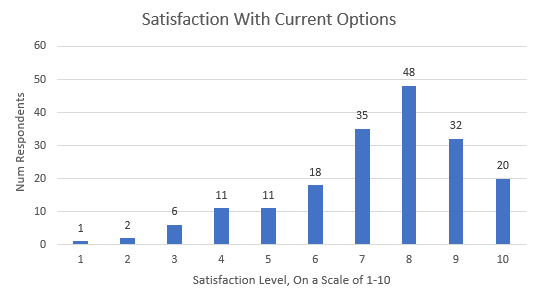
\includegraphics[width=.9\linewidth]{./images/satisfaction.PNG}
\end{center}

If we take satisfaction ratings of 7 or above as "generally satisfied" and 6 or below as "generally unsatisfied," then 49 out of the 184 respondents (26.6\%) are generally unsatisfied with current options. While not overwhelmingly negative, this is not the sort of response one would expect if there was not room for improvement.

\subsubsection{To combat the lack of open source, \emph{customizable} software}
\label{sec:orgd41c619}

This section will use the present state of Greek text input as an example to illustrate how customizable software is currently lacking. Similar situations and observations hold for other languages, but will not be discussed for brevity's sake. \\

\noindent \textbf{Current options for Greek text input} \\

The survey mentioned above contained questions about program usage in an attempt to get an idea of what tools Greek scholars/students generally use to type Greek.

\begin{center}
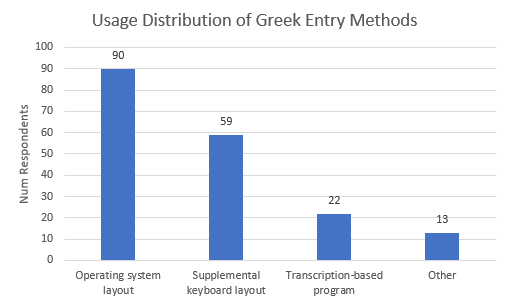
\includegraphics[width=.9\linewidth]{./images/entry-methods.PNG}
\end{center}

\begin{center}
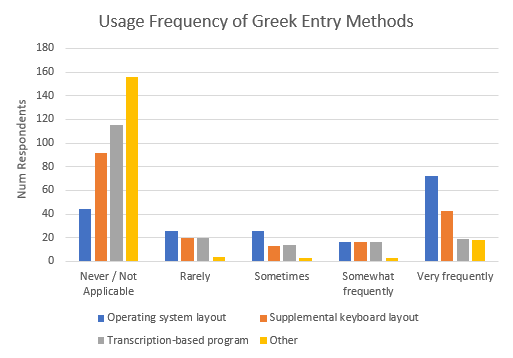
\includegraphics[width=.9\linewidth]{./images/entry-method-usage-distribution.PNG}
\end{center}

Most people either use a default operating system layout (e.g., Windows 10's Polytonic Greek layout) or a keyboard program that gives access to system-wide keyboard layouts (e.g., GreekKeys\footnote{\url{https://classicalstudies.org/publications-and-research/about-greekkeys-2015}}). Some people use transcription-based programs that employ something like Betacode to match up English and Greek (e.g., SophoKeys\footnote{\url{http://benjaminblonder.org/sophokeys/}}), and some people use something else completely, like multilingual word-processing programs (e.g., Yudit\footnote{\url{http://yudit.org/}}, da Grunk\footnote{\url{http://www.benwolkow.com/daGrunk/grunk-0.8.html\#daGrunk}}). Typegreek.com\footnote{\url{http://www.typegreek.com/}} and Antioch\footnote{\url{http://www.users.dircon.co.uk/\~hancock/antioch.htm}} were two of the more frequent "other" options on the survey. \\

\noindent \textbf{Positive characteristics of existing options} \\

Among different options one can observe several important design characteristics. Most of the solutions are \emph{homophonic}, meaning that alpha is put on the A key, beta on the B key, and so forth:

\begin{center}
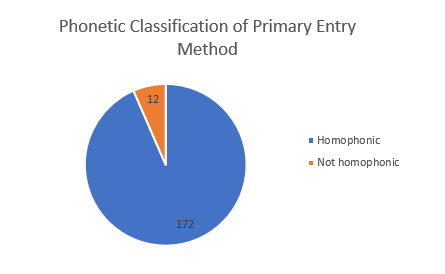
\includegraphics[width=.9\linewidth]{./images/homophonic.PNG}
\end{center}

Some (e.g., da Grunk) attempt to avoid complex chord sequences when entering diacritical marks by using punctuation-based mnemonics, and allow for flexible entry order, meaning that breathing-then-accent or accent-then-breathing (for example) both correctly display. Many (e.g., GreekKeys, SophoKeys) allow for text entry across applications rather than having to copy and paste out of some "special" window. All of these things are definite positives for a typist, especially one switching into Greek text entry from time to time while primarily typing in his/her native language(s). \\

\noindent \textbf{Customization and open source} \\

However, users who wish to customize things are out of luck with present options. Some people may wish to change how diacritics are handled, for example, or to change which Latin-script letter chi goes on to conform to their preferences (both C and X are popular, but it can be irritating to have to deal with both mappings). Because current options are closed source without significant customization interfaces, this is simply not possible.

Customization and open source software go hand-in-glove, and especially for a program such as this -- which is dealing with a very domain-specific problem that contains much that is subjective and/or related to user preference -- there is significant benefit to making software community-driven. Setting up a community-driven environment to create a customizable and open source framework for text entry of non-native languages is the primary goal of this project. \\

\noindent \textbf{Alternate keyboard layouts} \\

Another reason for this project's focus on customizability is the fact that currently available homophonic layouts (at least those that function at the system level) do not work for "nonstandard" keyboard layouts -- they all assume a QWERTY base mapping.

People typing on Dvorak, Colemak, QWERTZ, BÉPO, and so forth may wish to have the benefits of homophonic letter layouts in their non-native languages while retaining their native base layout. For this project, all of the functionality in any language can be implemented on whatever base layout is desired, with full customization as an option; while time constraints mean that only QWERTY will be supported out of the box initially, the underlying structure of the mapping does not rely on QWERTY, and other layouts should be supported in the future.\footnote{Different physical layouts for keyboards will also be supported eventually. Most people type on the standardized ANSI and ISO keyboards, but those who type on things like the Kinesis Advantage or Ergodox -- keyboards that have more keys to work with -- will not have to go through extra steps in customization once the physical configurations are supported.}

\subsubsection{To combat the lack of software that bundles multiple language layouts together}
\label{sec:orgbbd7f70}

This software is being developed in close association with Classicists, and the initial project scope is targeted at solving the problems of Greek scholars in this field. However, the project aims to create a framework that may be comfortably extended to other languages and alphabets as needed.

Some academic fields (e.g., Historical Linguistics, Classics, Ancient Near East, and Ancient History), have significant language demands. It is not uncommon for people studying in these fields to pick up multiple ancient languages (including, but certainly not limited to, Latin, Greek, Hebrew, Arabic, Syriac, and Sanskrit), with many of these having complex alphabets. A lack of consistency in approaches can be frustrating, particularly if one has to go through the bother of individually installing and updating text entry solutions for all these languages on all the computers used for writing.

Additionally, much secondary scholarship in these fields is in German, French, and Italian, all of which share the basic English character set, but demand a few special characters and/or accents. It is conceivable for a scholar working on research about Mediterranean trade in Late Antiquity, for example, to need to type in English for their core analysis, Latin, Greek, and Syriac for primary sources, and German, French, and Italian for secondary sources. Assuming Latin is typed without macrons and accents, that leaves 5 additional languages on top of English that must be dealt with.

While it is more a future goal than a priority of "round one" of this project, bringing multiple language layouts together in the same program is one of the central motivations behind creating another project dealing with these things. Starting from scratch rather than adding on to an existing program ensures that there will be seamless interoperability in the future, and that standards and design guidelines may be established.

\subsubsection{To combat the lack of software that adds functionality without removing any}
\label{sec:orgb4181c2}

Using keyboard shortcuts can be a frustrating experience when you have to type in another language. If there is no intelligent handling of modifier keys, people typing in a non-native language might miss such shortcuts as Ctrl-C (copy), Ctrl-X (cut), Ctrl-V (paste), Ctrl-Z (undo), and Ctrl-S (save). The situation is especially bad for those who use Vim, Emacs, or other text editors that make use of the keyboard (rather than a GUI) for functionality, and for people who use keyboard-driven window managers, browsers, application launchers, window switchers, and so on.

It can also be frustrating to "lose access" to some English keys (typically punctuation such as brackets) when typing in another language. If a language layer "steals" English punctuation keys thinking that they will never be needed when typing that language, but does not provide any way to access said keys short of disabling the software temporarily, it can create an unpleasant user experience.

Things like these are not the most obvious design factors when one thinks of typing in non-native languages, but they too are an important part of creating options for text input that are both pleasant and intuitive to use.

\section{Section 2: Nuts and bolts}
\label{sec:org5101844}

Before getting into this project in particular, it is proper to briefly examine the nuts and bolts that make multilingual text input a possibility on modern operating systems. Much more could be written about any of the things here, but the present section will seek only to provide a sufficient amount of background to give readers an appreciation for the complexity at play behind the scenes.

\subsection{Keyboard layouts}
\label{sec:orgc031cca}

To be able to type in a language that is not the default for your physical keyboard and system layout (e.g., a QWERTY ANSI keyboard used for American English), a different keyboard layout is necessary. In essence, a keyboard layout translates presses of physical keys into characters or key events (like Enter or Tab).\footnote{To be more precise, keyboards send signals that are interpreted by the operating system. Depending on permissions, different programs can inject themselves into the input system, and intercept keypresses before they get sent to other programs. This is what allows a remapping program to change the behavior of sent keys: the signals sent by the physical keyboard are the same, but they are intercepted and replaced with so-called "virtual keys" that lead to different behavior.} Most multilingual keyboard layouts today transform physical key presses directly into Unicode output, which is discussed in the next section.

It is helpful to think of the keyboard layout as the interface between users and languages on their computers: while a user may be competent at speaking/writing a language, and the computer competent at representing/displaying the language, if there is not a way for the user to input text, both of these things come to naught. Without an interface for users entering text into a computer, the language prowess of both the user and the computer are ultimately irrelevant.

\subsection{Unicode}
\label{sec:org860216d}

Unicode is a standard that defines character values based on underlying numerical representations. The specifics of this are not relevant for the purposes of this project, but it is important to note that there is not special significance to Unicode's definitions: all the numerical values that represent characters are essentially arbitrary. What makes Unicode useful is its standardization: by providing an agreed upon (if sometimes debated) correspondence from low-level computer encodings to characters, Unicode enables people of all languages have an unambiguous text representation that does not conflict with the text representations of other languages. Among other things, this lets different languages be typed side by side seamlessly.

\subsubsection{Precomposed and decomposed Unicode}
\label{sec:org91eed39}

Unicode essentially comes in two flavors: precomposed and decomposed. At a high level, precomposed Unicode represents letters with diacritics as individual characters, while decomposed Unicode represents letters with diacritics as a sequence of characters: one character for the letter, another character for the first diacritic, a third character for the second diacritic, and so on. For example, an epsilon with smooth breathing and an acute accent (ἔ) would be represented by precomposed Unicode as one character, while it would be represented by decomposed Unicode as three characters (epsilon + combining smooth breathing + combining acute accent).

As time has passed, the Unicode consortium has gotten more and more reserved about adding additional precomposed characters.\footnote{See \url{http://unicode.org/pending/proposals.html}: "Often a proposed character can be expressed as a sequence of one or more existing Unicode characters. Encoding the proposed character would be a duplicate representation, and is thus not suitable for encoding."} After all, so the reasoning goes, combining diacritical marks are already supported in the Unicode specification. Why should Unicode have to support "redundant" precomposed characters if you can just enter the same character as a sequence with combining characters?

The logic is fine so far as it goes, but the problem is that the Unicode text encoding is only half of the picture: without fonts that properly support decomposed sequences, decomposed Unicode is not really an option. There have historically been many problems with fonts improperly displaying combining characters. For example, the combining characters might be horizontally off-center compared to the letter, the vertical spacing between the letter and the diacritic might be too little or too much, multiple combining characters might overlap with each other, or not stack properly, and so forth.

Because different base characters have different physical characteristics (e.g., some are taller or wider or have ascenders and descenders to deal with) there is no cookie-cutter solution for physically placing combining characters. Rather, it must be done for each letter individually.

As will be discussed below, there are actually modern fonts that handle decomposed Unicode well. However, there are still plenty of fonts that do not, especially when you start combining multiple diacritics, or using any uncommon diacritics.

\subsubsection{Combining multiple diacritics}
\label{sec:org8c1f76c}

An additional wrinkle in decomposed Unicode with multiple combining characters is the entry sequence. What happens if you type all the permutations of three different diacritics -- do they all display the same?

The answer will typically be no. In the second chapter of the Unicode 11 manual, section 11 deals with combining characters, and discusses the default combining behavior for multiple combining characters:

\begin{quote}
By default, the diacritics or other combining characters are positioned from the base character’s glyph outward. Combining characters placed above a base character will be stacked vertically, starting with the first encountered in the logical store and continuing for as many marks above as are required by the character codes following the base character. For combining characters placed below a base character, the situation is reversed, with the combining characters
starting from the base character and stacking downward.
\end{quote}

A full discussion of multiple combining diacritics for Greek specifically can be found at \url{http://www.opoudjis.net/unicode/unicode\_ordering.html}.

\subsection{Fonts}
\label{sec:org6044a2d}

In recent years, font support for decomposed Unicode has improved significantly. In particular, support for so-called "smart fonts" (such as OpenType fonts) has improved to the point where most users will not have to concern themselves about whether or not their fonts play nice with decomposed Unicode so long as they are using popular mainstream fonts (Lucida Grande, Palatino Linotype) or common academic fonts for their language(s).\footnote{See \url{https://gervatoshav.blogspot.com/2015/07/greek-fonts-free-productivity-apps-and.html} and \url{http://www.russellcottrell.com/greek/fonts.asp} for good discussions of Greek font options. Domain specific fonts (such as the SBL fonts) will not support as wide a range of characters -- the IPA blocks, for example -- as more general fonts that have broad coverage (such as Cardo).} Mastronarde (2008), on pages 26-28, includes a good discussion of how fonts behave with smart features vs. how they behave without smart features, and has a helpful chart illustrating why smart features are to be desired. Of course, this is somewhat an application-level problem as well, since if an application does not support OTF fonts, for example, it will not support decomposed Unicode either (or at least is not likely to display it cleanly).

With all this having been said, even smart fonts can fail to handle some of the less common combinations. Macrons prove problematic in many otherwise excellent Greek fonts, for example, since there are not precomposed forms for combinations like macron + acute accent, and since decomposed macron + accent forms do not always display nicely. The path to fixing such problems is not always clear (since it might require the coordination of font designers, input system developers, and the developers of word-processing software), but usually there is a way.\footnote{A good example of font changes that can be undertaken to solve such problems can be seen in a series of blog posts by James Tauber, starting with this post: \url{https://jktauber.com/2016/01/28/polytonic-greek-unicode-is-still-not-perfect/}}

\section{Section 3: The Unicode Language Layers project}
\label{sec:org4a5d6ff}

Thus far this paper has examined exactly what this project is interested in at a high level (§1), and the sorts of details that must be dealt with when working with multilingual input on computers (§2). This section will seek to present a brief summary of this project's main goals and features.

\subsection{Sane defaults combined with ease of use}
\label{sec:org126b1e1}

Any software that users interact with directly must necessarily deal with considerations of the user interface (UI) and user experience (UX). Software (particularly that not targeted at experienced computer users like programmers) should be easy to download, install, run, update, and, most importantly, use. If software has a poor UI and UX, and is consequently difficult to use, it is not nearly as beneficial to users as it could potentially be.\footnote{While this statement is mostly self-evident, companies and organizations do exist to research and advise others on more specific matters of usability, UX, and UI. For example, \url{https://www.nngroup.com/}.}

One notable component of UX design is the so-called "principle of least astonishment" (or "rule of least surprise"). \emph{The Art of Unix Programming}, succinctly defines the principle as "In interface design, always do the least surprising thing,"\footnote{Section 1.6.10, p. 20. Cf. also Section 11.1 "Applying the Rule of Least Surprise," p. 254ff.} and \emph{Principles of Computer System Design: An Introduction} defines it as "The design [of a system] should match the user's experience, expectations, and mental models."\footnote{Section 2.3, p. 85.} In other words, programs should be designed so that they behave consistently (both internally, and with regards to common practices/standards), and do not violate user expectations.

This particular keyboard project does not have a graphical frontend, but does make use of the principle of least astonishment in its design of language layouts and diacritic behavior. The general idea is to create defaults that will make sense to most people, and to structure program behavior around "normal" patterns of both language use and computer use.

\subsection{Letter placements that make sense}
\label{sec:orgf1e7a79}

Since this project is targeting the typing of non-native languages (see §1.1), letter placements should be intuitive for typists that are not typing in a language frequently or for a long time. The survey data gives a good graphical representation of such usage:

\begin{center}
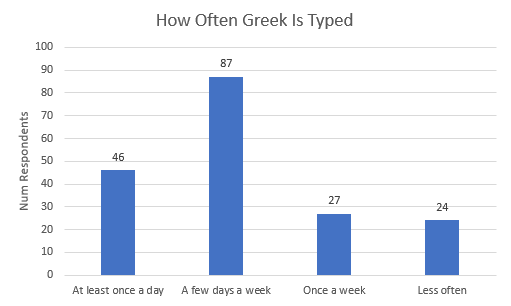
\includegraphics[width=.9\linewidth]{./images/typing-frequency.PNG}
\end{center}

\begin{center}
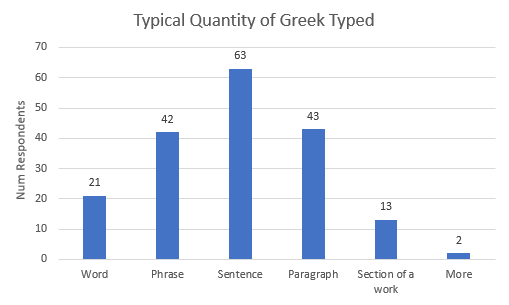
\includegraphics[width=.9\linewidth]{./images/typing-quantity.PNG}
\end{center}

Because long blocks of non-native text are not being typed often, this project makes design decisions that favor memorability over raw optimality.

\subsubsection{Typing performance and keyboard layout considerations}
\label{sec:org08e3908}

Studies of typing have identified some trends in terms of keystroke efficiency and general typing performance. For example, Dhakal \emph{et al.} (2018), in a study of 168,000 volunteer typists, found that inter-key intervals (IKIs) -- the time intervals between subsequent key presses, a good predictor of overall typing speed -- were lower for bigrams (two-letter sequences) that alternated hands (i.e., had one letter typed by one hand, and a following letter typed by the other hand) than for bigrams typed on only one hand. Feit \emph{et al.} (2016), in their overview of previous studies of typing, summarize well established phenomena and their corresponding measures based on prior studies of professional touch typists; the finding reported above has been noted multiple times in prior studies. Additionally, it has been observed that repeated key presses have lower IKIs than same-hand key presses (with keys pressed by different fingers), which in turn have lower IKIs than keypresses that require the same finger to press two different keys in succession.

Dhakal \emph{et. al} (2018) also found that faster typists make/need to correct fewer mistakes than slower typists, that faster typists use more fingers on average, and that faster typists have high "rollover percentages" -- a measurement of how many keystrokes begin with other keys already being pressed down from a previous keystroke. Feit \emph{et al.} (2016) observed a similar phenomenon in that they came to the conclusion that the preparation of keystrokes leads to lower average IKIs. They also noted that a lower standard deviation in global hand position (i.e., lower overall hand movement from some "home position") similarly leads to lower average IKIs, and that a consistent key mapping of finger-to-key ("low entropy") has a similar effect.

Pulling these observations together, one arrives at something like the following:

\begin{itemize}
\item Bigrams involving hand alternation are faster (in terms of low IKIs) than repeated keypresses (i.e., a bigram with only one unique key pressed twice by the same finger), which in turn are faster than (non-same-finger) same-hand bigrams, which in turn are faster than (non-repeated) same-finger bigrams.
\item The ability to "prepare" following keypresses positively associates with typing speed (low IKIs), which helps explain why fast typists have high rollover percentages: lining up future keystrokes makes it easier for fast typists to have multiple keys down at the same time.
\item Low overall hand movement positively associates with typing speed (low IKIs). This is likely mediated through low-movement typists being better able to line up future keypresses.
\item The number of fingers used to type positively associates with typing speed (words per minute: WPM).
\item A low error rate positively associates with typing speed (WPM).
\item A consistent mapping of finger-to-key ("low entropy") positively associates with typing speed (low IKIs).
\end{itemize}

Mapping these observations onto keyboard layout design is not exactly 1:1. The above studies had populations of almost entirely QWERTY typists. QWERTY heavily loads the left hand, and does not actually favor a neutral hand position on the home row since very frequent letters such as e, t, r, o, i, n, etc. \{cite Mayzner in footnote\} are not actually on the home row. (This would have the net effect of actually \emph{penalizing} people that learned a 10-finger touch typing system that teaches slavish hand positioning on the home row). Moreover, the second study did not have any typists above 79 words per minute, which is below the \emph{average} 80+ WPM typing rates of earlier studies that focused on trained, professional touch typists (on typewriters, no less, which disallow rollover by mechanical design). For these reasons, I do not agree with the conclusion of this study that touch-typists (defined as people able to type without looking at the keyboard to find keys) and non-touch-typists have similar typing speeds on a philosophical level: perhaps for the suboptimal QWERTY layout for typists of slow to average speeds, but not in general, and almost certainly not for typists on right tail of the distribution, with speeds exceeding 120 WPM. In other words, while I do think that the study is valuable in that it shows that most average typists won't benefit from a structured system, I do not think it says anything about the usefulness of the structured system as one approaches higher speeds, particularly on more intentionally designed keyboard layouts.\footnote{Full disclosure: I type on an algorithmically generated custom layout (with heavy automation built in: autospacing of punctuation, autopairing of parentheses etc., autocapitalization, and so forth), and have spent a great deal of time over the years thinking about these things. See \url{https://github.com/StevenTammen/hieam}.}

Additionally, it is somewhat difficult to map things like "low error rate" onto keyboard layouts. Perhaps some keys are more easy to confuse than others, and some sequences of keypresses are harder on a physiological level, but these things are difficult to measure, and may vary widely by individual.

With all this being said, present data does support prioritizing bigram hand alternation, prioritizing low overall hand motion, and minimizing the amount of consecutive non-repeat keypresses involving the same-finger.

\subsubsection{The design of non-native keyboard layouts}
\label{sec:org10cc352}

Given the above discussion, one might wonder if it is worth designing keyboard layouts for non-native language that try to minimize IKIs and maximize WPM by their very design. Once in muscle-memory, they would certainly allow for higher theoretical speeds.

However, the exceedingly great complexity of the cognitive processes behind typing -- see Rumelhart \emph{et al.} (1982), e.g., for a specific proposed model-- makes it difficult to pin down performance causalities, particularly with respect to mental models of keyboard layouts. For example: what effect do semantic groupings of characters have?

As a general rule of thumb, so-called "fully optimized" layouts (which tend to have high hand alternation, low overall hand movement, and low same-finger) will have relatively poor inherent memorability in terms of semantic groups. If you lets a genetic algorithm design an optimized layout for you, it will not keep all the letters in a block or numbers in a row, but mix everything together according to frequency considerations. We humans are very pattern-oriented creatures, and having no apparent structure to characters will inevitably make a keyboard layout more difficult to remember, to some degree. Furthermore, it would seem likely that keyboard layouts that are easier to remember will be easier to get up to speed with, especially if you don't practice with them very much.

The issue in all this is that there is not any research that explicitly covers these things.\footnote{At least not any research that I am aware of at the time of writing. It is possible that someone has studied these things in a less formal way, and not published their results.} For this reason, it is impossible to say definitely how much easier semantically-grouped keyboard layouts for non-native languages are to learn than fully-optimized keyboard layouts for these same languages, or how much faster people may train them to, say, 35 WPM. The data for this simply does not exist. However, this paper is operating on the assumption that these considerations are non-negligible for most people in most circumstances. The hypothesis coming from such an assumption is this: since people typing non-native languages will not be typing them with great frequency and magnitude, it is more rational to focus on memorability over raw optimization considerations, since layouts that are easier to remember will be faster to learn, and the benefits of "brute forcing" an optimized layout (as one might do for one's native language) will never be realized in typical use cases.

\subsubsection{Native-language layouts in muscle memory}
\label{sec:org6d295de}

The above discussion focused on the interplay of memorability, layout optimality (as measured by hand alternation, overall hand movement, same-finger, etc.), and ease of acquisition in the abstract. However, assuming users of this project can already type on a keyboard layout in their own language (in whatever regard: touch typing, hunting and pecking, etc.), people are not starting from ground-zero.

The general idea is that for the circumstances under which most people type non-native languages it is \emph{always} better to associate a keyboard layout for a non-native language with a keyboard layout for a native language already in muscle memory. Associating a new layout with the old layout lets typists reuse neural pathways that are already in place rather than forming new ones from scratch.

What does this mean? Let's take the Greek letter alpha. Most people, Classicists or no, know that alpha corresponds in phonetic value to the English letter A. Alpha also happens to look like the letter A in both its lowercase and uppercase forms. So, rather than putting alpha on some random key, why not simply place it on the same key as the letter A in English?

\subsubsection{Issues in constructing associations}
\label{sec:org6b723a5}

If we accept the premise that it is best to form correspondences between non-native languages and keyboard layouts already in use (for English or otherwise), then it follows that we need some formalized system for doing so.

Layouts derived from phonetic matching are typically called "homophonic layouts." While homophonic layouts are excellent when correspondences exist, there are some letters in languages that have no clear English equivalent. Theta in Greek, for example, corresponds to the phoneme in English that is represented by the digraph "th." These must be dealt with separately.

The association (henceforth keymap, short for "key mapping") below for Greek attempts to solve such issues in a systematic way. Following the hypothesis presented above (namely, that memorability is a more important concern in these circumstances than raw optimality), priority is given to phonetic correspondences, then visual correspondences, then transcription correspondences, then, finally, to raw optimality.

The ordering of priority above is not based on any hard data (as no such data exists at present, as above), but based on the principle of least astonishment and logical consistency:

\begin{enumerate}
\item Following the principle of least astonishment, if "most" keys are being placed by phonetic correspondence, it makes sense to use phonetic correspondence as the primary determiner of non-native character position, wherever possible.
\item Following this, visual correspondences are used since they do not depend on any particular system (unlike transcription correspondences, which may only "work" for some transcription schemes), and also have greater "astonishment factor" for alternate keymaps than transcription correspondences (particularly in the case of Greek, which shares many graphemes with English in lowercase and especially uppercase forms). For example, eta in Greek is almost universally put on the letter H in keyboard layouts, since capital eta \emph{is} the grapheme H.
\item Transcription correspondences come next, in that they are a better mnemonic than nothing. Transcription correspondences work best for letter-based transcription (i.e., transcription that does not involve the used of special diacritics), especially that involving only single graphemes. A good example of this is using Q for quf on Hebrew keyboard layouts: the English letter Q most certainly does not take on the phonetic value [k], but since quf is very commonly transliterated as Q, it is easy to associate the letter Q with quf.
\item Finally, raw optimality is used when none of the mnemonics work. The letter theta in Greek, for example, has no phonetic \emph{letter} equivalent in English (even though we use [θ] all the time), has no letter look-alikes, and is commonly transliterated as th or tʰ, which doesn't help create any good associations (since tau makes the most sense for the English letter T). So theta is placed on a key that performs best with respect to the goals of high hand alternation, low overall hand movement, and low same-finger.
\end{enumerate}

\subsection{Example: Greek letter placements}
\label{sec:org00ae414}

\subsubsection{Phonetic correspondences}
\label{sec:org23c6621}

Greek is a challenging language to pin down phonetically inasmuch as it has undergone a great deal of change. Even if one limits the time of interest from c. 800 BC to c. 200 AD, the language underwent substantial change. A good book for getting a handle on Greek phonetics is W. Sidney Allen's \emph{Vox Graece: A Guide to the Pronunciation of Classical Greek} (1999, 3rd ed.). At different times and different places Greek was pronounced differently. So "which Greek" should form the phonetic basis for the layer correspondences? It is a challenging question.

Most discussions revolve around theta and phi. In later Greek, theta and phi were definitely pronounced as fricatives (as [θ] and [f], respectively). In early Attic, however, they were pronounced as aspirated stops. This much is uncontroversial. The question is which pronunciations should be used in the classroom, and by extension here, which pronunciations should be used in constructing phonetic associations for a keyboard layout?

I think there are good pedagogical arguments for both pronunciations. Native English speakers have a very hard time distinguishing between aspirated and unaspirated stop consonants (either voiced or voiceless) since they are never different phonemes in English (unlike, say, Hindi/Urdu). This makes using the fricatives attractive inasmuch as students are much less likely to mis-spell and mis-identify words involving tau/theta or pi/phi. However, Attic is the dominant dialect taught (outside of New Testament circles), and early 4th century Attic (e.g., Plato) with [θ] and [f] is simply incorrect from a historical perspective.

This project does not pretend to settle this debate, but simply uses [θ] and [f] for the pronunciations of theta and phi because doing so is expedient: eliminating phonetic overlap (from the English perspective) makes a phonetic mapping less ambiguous. Purists will forgive me, I hope.

If a letter has any English equivalent (even if it has additional sounds in some contexts not found in English, as with gamma being pronounced as [ŋ] before velars), I have opted to match them. I have also opted to match "near misses" -- sounds that aren't quite identical (or at least are not so on an exact 1:1 level), but are close enough that they are obviously connected (such as rho and R, and many of the vowels). I have chosen to pass over letters that could be considered ambiguous in terms of phonetic correspondences (e.g., omicron/omega/O, epsilon/eta/E, kappa/chi/C/K, etc.), so that further matching may be accomplished (through visual correspondences, e.g.) without any arbitrary decisions being made. Here are all the matches that follow from this:

\begin{center}
\begin{tabular}{lll}
Greek letter & IPA & English match\\
\hline
Α α & [a], [aː] & A\\
Β β & [b] & B\\
Γ γ & [g], [ŋ] (before velars) & G\\
Δ δ & [d] & D\\
Ε ε & [e] & \\
Ζ ζ & [zd] & Z\\
Η η & [ɛː] & \\
Θ θ & [θ] & \\
Ι ι & [i], [iː] & I\\
Κ κ & [k] & \\
Λ λ & [l] & L\\
Μ μ & [m] & M\\
Ν ν & [n] & N\\
Ξ ξ & [ks] & X\\
Ο ο & [o] & \\
Π π & [p] & P\\
Ρ ρ & [r] & R\\
Σ σ & [s] & S\\
Τ τ & [t] & T\\
Υ υ & [y], [yː] & U\\
Φ φ & [f] & F\\
Χ χ & [kʰ] & \\
Ψ ψ & [ps] & \\
Ω ω & [ɔː] & \\
\end{tabular}
\end{center}

This "first pass" at matching gets us pretty far, but there is still some work to do. There are basically two kinds of letters that have not been matched at this point: those that are ambiguous in terms of phonetics (ε/η, κ/χ, and ο/ω), and those that have no English phonetic equivalent (θ, ψ)

\subsubsection{Visual correspondences}
\label{sec:org62e026e}

Look-alike letters, even if they have no phonetic correspondence, can be an easy way to remember letters. Anything that helps create mental associations can help speed up the learning process. Both uppercase and lowercase forms are considered.

\begin{center}
\begin{tabular}{ll}
Greek letter & English match\\
\hline
Ε ε & E\\
Η η & H\\
Θ θ & \\
Κ κ & K\\
Ο ο & O\\
Χ χ & \\
Ψ ψ & Y\\
Ω ω & w\\
\end{tabular}
\end{center}

Uppercase epsilon, eta, kappa, and omicron look identical to the uppercase English letters E, H, K, and O, respectively (and lowercase omicron also looks identical to  lowercase O). Furthermore, lowercase omega looks very similar to lowercase W. Uppercase psi looks similar enough to uppercase Y that it is worth using as a mnemonic, in my opinion. Note that while chi looks very similar to the English letter X, we are already using X to represent xi.

This second round leaves us with only two letters remaining: theta and chi.

\subsubsection{Transcription correspondences}
\label{sec:orgfe4e339}

One of the problems with transcription is that it is not terribly standardized, and where standards exist, they exist in plural. An excellent treatment of Greek transcription/transliteration standards comes from Verbrugghe (1999), who identifies five main schemes: Latin transcription, Beta Code transliteration, Latin transliteration, Modern Greek transcription, and Modern English transcription. Here are our letters of interest in each of the five schemes:

\begin{center}
\begin{tabular}{llllll}
 & Latin & Beta Code & Latin & Modern Greek & Modern English\\
Greek letter & transcription & transliteration & transliteration & transcription & transcription\\
\hline
Θ θ & th & q & th & th & th\\
Χ χ & ch & x & ch & h & kh\\
\end{tabular}
\end{center}

Of these five schemes, Beta Code transliteration (used by TLG and Perseus) and Latin transliteration are not really used in representing Greek text outside of search boxes, at least in the modern day. Modern Greek transcription is not sufficient for transcribing ancient Greek, and so is not of interest for this particular implementation. This leaves us with Latin transcription and Modern English transcription.

Latin transcription has been around in some form since the time of the Romans, and for better or for worse, many English words that have Greek origin are almost universally used in the form of their Latin transcriptions. Modern English transcription, on the other hand, is more concerned with closely mirroring the underlying Greek forms and pronunciation (free from the influence of the Latin language and Roman culture). A prime example of the differences may be observed in the transcription of Ἀχιλλεύς: most English speakers would recognize "Achilles" as the Greek hero of the \emph{Iliad}, but fewer would be able to recognize "Akhilleus," even though it is a much more accurate representation of the underlying Greek.

For our purposes, it is enough to note that ch is a fairly common transcription used of chi (especially in less scholarly circles), and that the letter C sounds like chi anyway. This is sufficient, in my mind, for putting chi on C, even though the mnemonics are not perfect. It is loads better than Beta Code's X, in my humble opinion. To this day I always enter searches wrong when using Beta Code, since I have never been able separate chi from C and xi from X in my head.

\subsubsection{Raw optimality}
\label{sec:orgf170715}

Theta is a tricky letter to place, since none of our correspondence efforts help with it. (I'm ignoring Beta Code's use of q for theta as it is entirely arbitrary and not useful as a mnemonic, in my opinion). English letters that are left include Q, V, and J.

None of these letters is particularly satisfying as a choice, but J is probably the best for people that type on QWERTY or its variants (like AZERTY, e.g.), since it is on the home row. For this reason, I have made it the default mapping for theta. People that do not type on QWERTY (Dvorak, Colemak, Workman, etc.) may want to alter this location, depending. I type on a custom layout and kept it on J because it was still the best location.

\subsubsection{Leftovers}
\label{sec:org7bd753b}

As to Q and V, I have these default to koppa and digamma, respectively. Both of these come from earlier forms of Greek that are closer to the Phoenician, but may be useful to type on occasion. For people that read on for the Hebrew keymap, koppa\textasciitilde{}quf and digamma\textasciitilde{}vav, so Q and V are actually logical choices given the Semitic consonants underlying these letters.

Digamma dropping explains the -ευς declension and the development of certain stems and words. For example, βασιληϝ- to Βασιλεύς, νηϝ- to ναῦς, βοϝ- to βοῦς, and so on. Koppa can be also be useful in explaining language development, as can the third and last early Greek letter: san. \{Todo: explain how to generate San\}

\subsection{Diacritic and punctuation placements that make sense}
\label{sec:orga000077}

Placement of diacritic and punctuation keys is one of the key areas that this project distinguishes itself from others. Many (but not all) keyboard layouts for languages like Greek use either dead-keys or complicated chords (Ctrl + Alt/Option + something) to enter diacritics, which is far harder to remember than a single key equivalence, particularly a key equivalence with visual correspondence. Single keys (even those that require shift to enter) are also much faster to type in general: while it is possible to reduce the IKIs between keypresses to some degree (see §3.2.1), an extra keypress will always be an extra keypress. Survey respondents overwhelmingly rated the single-key method of entering diacritics as their first choice:

\begin{center}
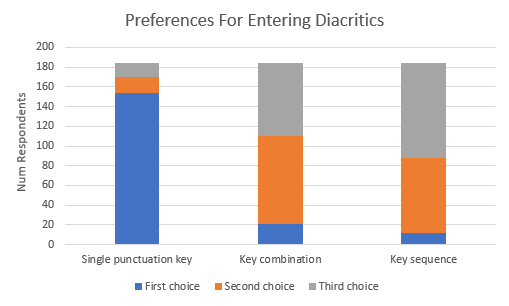
\includegraphics[width=.9\linewidth]{./images/diacritic-entry-preferences.PNG}
\end{center}

Since diacritics don't have phonetic value or any transcription equivalencies most of the time, finding memorable places for them relies comparatively more on visual correspondences and raw optimality. The visual correspondences are a little less obvious as well (e.g., : yields a diaeresis as apposed to a yields α). However, there is another variable at play here that was not present for letters: semantic correspondences. If different languages use different symbols to indicate questions, exclamations, pauses, and so forth, an obvious mnemonic is matching keys based on similar sentence function. In many ways this is the "phonetic matching of punctuation," inasmuch as keys are being matched directly based on expected usage (i.e., according to the principle of least astonishment).

According to these observations, priority is given to semantic correspondences, then visual correspondences, and then to raw optimality. Note the similarities to the order of priority for letters: in many ways, we are running through the exact same procedure for a different class of characters.

\subsection{Example: Greek diacritic and punctuation placements}
\label{sec:org5f802e2}

\subsubsection{Establishing available keys}
\label{sec:org57b0d1c}

Greek has a variety of diacritics that are an essential part of the language. According to our plan of putting these diacritics on English punctuation keys, it is necessary to figure out which punctuation keys are "free" when typing in ancient Greek. It would be possible, of course, to use "already taken" punctuation keys for diacritics, but that would require very frequent use of the language leader key to access the actual punctuation. For this reason, I have opted to only consider punctuation keys that are not themselves typically used in Greek.

\begin{center}
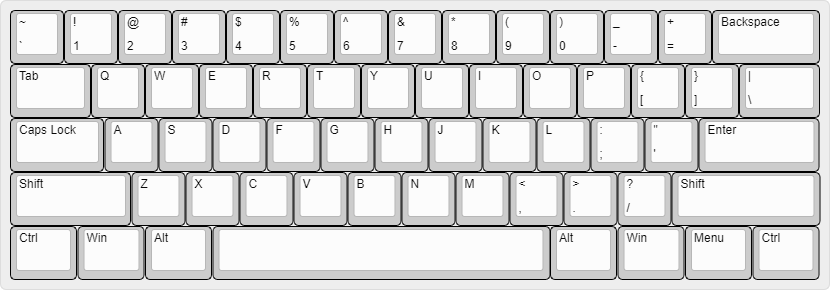
\includegraphics[width=.9\linewidth]{./images/base.png}
\end{center}

This is the ANSI 104 key layout with the function keys and right side of the keyboard (arrow keys, number pad, etc.) removed to save space. This physical layout is very common in the English-speaking world, and will be the one used in all discussions of key placement from here forward.

\begin{center}
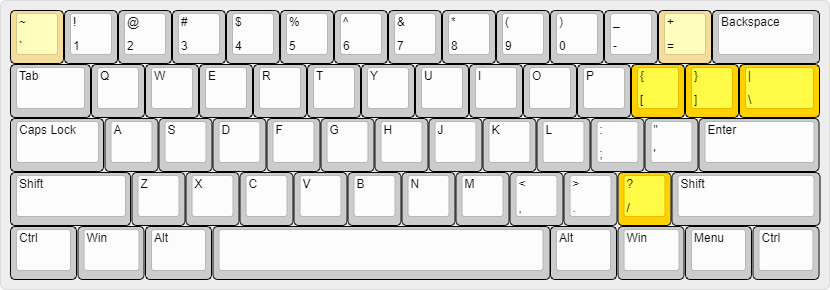
\includegraphics[width=.9\linewidth]{./images/unused-no-shift.png}
\end{center}

This image highlights unused punctuation keys that do not require shift. Numbers are ignored so that they may typed regularly if wished (and to stay consistent across languages). Note that the semicolon is ignored here as well, for the moment, since it is "used" as the Greek question mark. We'll return to it later. The apostrophe and hyphen both have uses (as a marker of elision and as an affix marker, respectively), so they have been excluded as well.

The two keys on the number row have been highlighted in a paler color, to indicate their relatively less favorable position. Keys on the number row require a great deal of hand movement to access, which makes them slower to type (see section §3.3.1).

\begin{center}
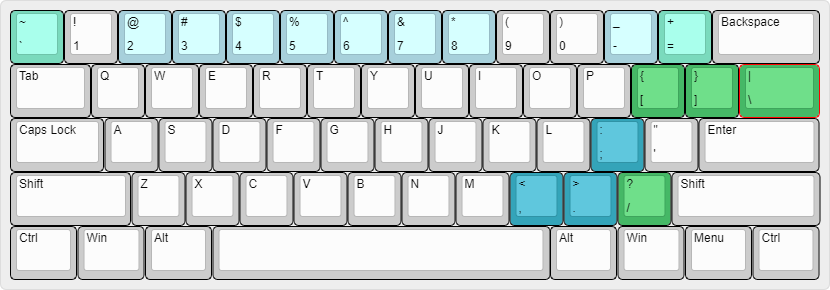
\includegraphics[width=.9\linewidth]{./images/unused-shift.png}
\end{center}

Finally, this image highlights the unused punctuation that do require shift. These keys are strictly inferior to those that do not (i.e., those from the above picture) since they require a whole additional keypress. Parentheses have been excluded since they are commonly used when writing ancient Greek (even if they do not show up in ancient sources), and the exclamation mark has also been excluded since it is not uncommonly used with imperatives.

Keys that have unused punctuation in both their unshifted and shifted states are shown in green, while those that only have unused punctuation in their shifted state are shown in blue. The shading distinction has been kept: the paler keys on the number row still indicate a relatively less favorable position. All of these keys are options that we can use for our diacritics and punctuation.

\subsubsection{Semantic correspondences}
\label{sec:orgc74177e}

Before turning to visual correspondences, it is worth considering direct semantic matches. Greek does not use the English question mark, but it does have a question indicator (the Greek question mark, which looks like a semicolon); similarly, Greek does not use the English semicolon, but it does have a way of indicating a half-stop (the Greek middle dot). It would be very confusing to use different keys for the same meaning, so the Greek equivalents are placed where their English counterparts are. Note that this \emph{is} somewhat confusing in that the semicolon visually represents the Greek question mark, but is mapped to Greek middle dot since that is the semantic equivalent to the English semicolon.

\begin{center}
\begin{tabular}{ll}
Punctuation & Semantic match\\
\hline
Greek Question Mark & ?\\
Middle Dot & ;\\
\end{tabular}
\end{center}

\subsubsection{Visual correspondences}
\label{sec:orgbf5ccb1}

Most of the rest of the diacritic keys can be placed directly using visual correspondences:

\begin{center}
\begin{tabular}{lll}
Grouping & Symbol & Visual Match\\
\hline
Breathings & Rough & [\\
 & Smooth & ]\\
Accents & Acute & /\\
 & Grave & $\backslash$\\
 & Circumflex & \textasciitilde{}\\
Quantity & Iota Subscript & \(\vert{}\)\\
 & Macron & \\
 & Breve & \\
Other & Diaeresis & :\\
 & Underdot & *\\
\end{tabular}
\end{center}

This leaves us with the macron and breve to place. Since these things are related, it would be nice to place them on a pair of keys. That leaves us with either \{ and \}, or with < and >. While all of these keys require shift to access (and so are similar with regards to raw optimality), the former are much more similar to the macron and breve in shape, and are thus used in this layout.

\subsubsection{Raw optimality}
\label{sec:org88f5fc7}

Note that the chosen keys not only match visually, but also make sense with regards to raw optimality. The most common Greek diacritics (including the breathings and the accents) are all accessible with a single key press without needing to use shift.

\subsection{Intuitive diacritic and backspacing behavior}
\label{sec:orgee379b7}

Unicode diacritics can be implemented in such a way that adding and removing them becomes complex and messy. For example:

\begin{itemize}
\item If precomposed Unicode is entered with stateless key combinations, adding or removing a diacritic to a letter that has already been typed involves deleting the entire last character and then pressing a new (correct) key combination.
\item If diacritics are entered by means of decomposed Unicode, display problems commonly occur if diacritics are entered in an incorrect order. For example, if a user types alpha then an acute accent, and then, a couple second later, decides that that alpha should also have a macron, he or she typically \emph{cannot} just press the diacritic key for the macron: due to how Unicode treats multiple combining characters (see §2.2.4), the accent will appear closer to the alpha than the macron, which is typically not the stacking behavior that is desired.
\item If diacritics are entered by means of decomposed Unicode, by default there is no way to change or remove diacritics any way but sequentially. That is, if you have something like alpha + smooth breathing + circumflex + iota subscript, and wish to either remove the smooth breathing or change it to rough breathing, you will have to delete all three diacritics to be able to change the breathing.
\item Etc.
\end{itemize}

This project abstracts all of the messy implementation details away from the user. In this project, diacritics are added to a letter by pressing the \emph{single} keys associated with them, typically linked mnemonically (see §3.1.4, above). They can be added in any order, but will always display correctly. They can also be removed in any order: pressing a diacritic key again when the diacritic is already on the preceding letter will remove it, \emph{regardless of the entry order}. Whether it was the last combining character entered or three back, it will still get removed while leaving all the other diacritics untouched. Finally, changing between options within a diacritic category that has mutually exclusive choices does not require deleting an old option before switching to a new option (although it still works seamlessly if you choose to do it this way). So, for example, if you had typed our sequence from above, alpha + smooth breathing + circumflex + iota subscript, but wanted to change that circumflex into an acute accent, all you would need to do is press the diacritic key for the acute accent. The circumflex would get deleted automatically, and replaced with an acute accent. These behaviors align with survey respondents' preferences to immediately see diacritics when typing them, which was generally ranked as the most important design consideration after layout memorability:

\begin{center}
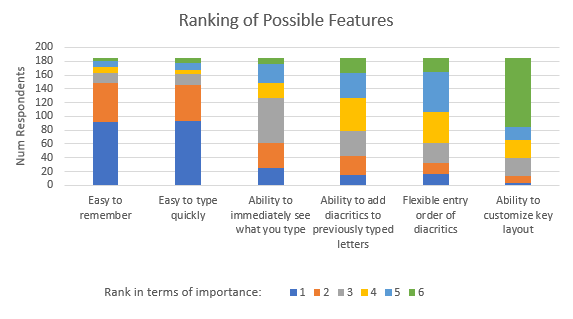
\includegraphics[width=.9\linewidth]{./images/ranking-of-possible-features.PNG}
\end{center}

These behaviors also allow for complete flexibility in entry order, which was another of the options. It was not as important to most people as immediately seeing diacritics as they are typed, but it was ranked 1st or 2nd by some individuals. "Smart" diacritic behavior that lets one add and remove diacritics from anywhere in a document was not implemented in the project, despite being one of the more valued features, since it is impossible to implement in a general, program-independent way.\footnote{Programs that let you change diacritics on the fly have some way to access the file/text object you are working on directly (i.e., have read/write permissions for the file on disk and have it open through the kernel, or have some equivalent mechanism on the web). However, such programs are not portable; you cannot go back and dynamically change diacritics if you are typing in an email client, for example, since the text box in the email client is not in the special environment that enables the file checking (lookbehind) necessary for on the fly diacritics.}

Handling individual removal of diacritics in the above manner lets Backspace function exactly how one would expect it to (in line with the principle of least astonishment): Backspace always deletes one full character. Within the bounds of this project, pressing Backspace once deletes one letter, regardless of the number of diacritics attached to said letter, instead of simply deleting the last diacritic typed.

\subsection{Minimal interference with normal computer use}
\label{sec:orga7185aa}

\subsubsection{The language leader key}
\label{sec:orgb1f35b2}

A challenge when dealing with multilingual language input is adding all of the additional functionality (switching between multiple languages, adding Latin-script diacritics for European languages, etc.) without compromising normal computer use in a significant way. Part of the reason for minimizing layout differences is to reduce change friction (the added time it would take to learn new key behavior), but a big part of it is also to avoid "losing" potential behavior by overriding keys. For example, if someone were to use the Function keys for switching between languages, that person would lose access to the Function keys themselves.

This project minimizes the impact of adding language behavior by encapsulating it all under a single key, henceforth the "language leader key." The language leader key is used to prefix other keypresses to change their behavior. In this way, the only key with changed behavior when typing one's native language is the key assigned to be the language leader key. This project uses CapsLock as the language leader key by default, since most people use it very infrequently and it is in a favorable position. Normal CapsLock behavior is not lost: one simply needs to press CapsLock twice instead of once to access it.

The language leader key is used for three main things: quickly switching between languages using mnemonics (e.g., language leader + g switches to Greek), quickly adding diacritics and special characters for European languages that otherwise do not need a separate layer\footnote{Recall that these languages are not being viewed as native languages. Native German speakers, for example, would definitely want ä, ö, ü, and ß accessible without the extra bother of using the language leader key as a prefix. Like the rest of this project, this particular behavior is targeted at people who wish to easily type \emph{non-native} languages (like an English speaker typing German words every once in a while).} (e.g., language leader + / adds an acute accent, language leader + c adds ç, etc.), and quickly entering punctuation on non-native layers when it is used for diacritics by default (e.g., ] adds smooth breathing by default for the Greek layer, but a closing bracket may be entered literally with language leader + ]).

\subsubsection{Consistent keyboard shortcuts}
\label{sec:orgabcdaee}

Most people are familiar with and use keyboard shortcuts like Ctrl-C, Ctrl-X, Ctrl-V, Ctrl-Z, and so on. Losing these when you are typing in a non-native language can be supremely irritating.

To be fair, it is possible to make keyboard shortcuts work in programs such as Microsoft Word when using an operating system layout. This project does not pretend to be the first that has ever made it easy to keep consistent keyboard shortcuts. However, this project does so out of the box, and does so for \emph{all} sorts of programs being used (including things like browsers and email clients).

\subsection{Customizability as a first order priority}
\label{sec:org7938a40}

\subsubsection{Layouts, layers, and languages}
\label{sec:org065f57a}

As mentioned in §1.2.1, customization is one of the main reasons for this project's existence. Other already existing programs allow for much of the same behavior as this project does, but do not allow for a very high degree of customization.

This project attempts to split low-level customization into clearly distinct categories that are easy to understand. When changing the base keymap (e.g., from QWERTY to Dvorak) or physical keyboard layout (e.g., from an ANSI 104 key keyboard to a Kinesis Advantage), one is working at the \emph{layout} level. When changing which language layers are included and what key sequences activate them, one is working at the \emph{layer} level. When moving letters around for a particular language or changing diacritic behavior, one is working at the \emph{language} level.

All three types of customization require different changes, and are documented separately. Together, they allow for very fine-grain control of the program and its behavior.

\subsubsection{Unicode send type}
\label{sec:org248e709}

It is not uncommon for multilingual keyboard layouts to use one predefined type of Unicode. Most layouts that use dead keys (e.g., the Polytonic Greek keyboard layout for Windows 10) send precomposed Unicode only.

This project lets users choose between precomposed and decomposed Unicode, and handles entry in exactly the same way. That is to say, how you add and remove diacritics (as described above) is consistent for both precomposed and decomposed Unicode, so you can freely switch between them without having to worry about different systems of entry.

\section{Section 4: Efficient Typing Practice and Greek Pedagogy}
\label{sec:org623b7e0}

\subsection{Repetition in typing}
\label{sec:org07a30f7}

Within any given language, some words (or parts of words: prefixes, suffixes, etc.) occur with much greater frequency than others. Over time, these words will be typed far more often than words which do not form as essential a part of the language's vocabulary. It follows that if one can learn how to type these words rapidly, their disproportionate occurrence within the language's corpus will lead to significant increases in overall typing proficiency (as measured by speed).

Chua and Liow (2014) conducted a study researching why people start spelling high-frequency words faster than low-frequency words. They note that "word frequency effects have been found in spelling-to-dictation with skilled adults such that participants are quicker to initiate spelling of high-frequency words than that of low-frequency words upon hearing the target stimuli." Their study attributes faster first-letter output for high-frequency words to three distinct phenomenon: spoken word recognition, orthographic retrieval, and response execution. Loosely speaking, these can be summarized in order as "figuring out which word, figuring out how to spell it, and figuring out how to translate the spelling into writing/typing movements." For the purposes of this project, it doers not much matter which phenomenon is most important for the faster speeds observed: the general idea is that higher-frequency words are processed faster.

Bannard and Matthew (2008) conducted a study researching frequently occurring "chunks" in child-directed speech, and what affect these stored word sequences have in the speech of children. While their study parameters are markedly different from Chua and Liow's study, the overall significance is similar: frequent sequences are repeated by children more quickly (and accurately) than infrequent sequences. This localizes some of the speed considerations to cognitive processing (i.e., identification of a word rather than lower-level translations of it into hand movements for writing or typing), but doesn't diminish the overall takeaway: it seems that language aspects of human cognition are conditioned by frequency considerations.\footnote{Many more related studies may be found in the discussions and bibliographies of both of the cited sources.}

These observation are in line with a conception of typing as a form of hierarchical control. Yamaguchi and Logan (2016) articulate a view of typing in which the translation of language into hand movements is governed by the development of "chunks." In the process of hierarchical control, something in an "outer-loop" of processing is mapped onto several "inner-loop" units (e.g., letters or keystrokes), thus chunking inner-loop units into an outer-loop unit. To use a Greek example, when someone is typing text from a paper source (to quote in research) and comes across the word συμβαίνω, they might first unconsciously split the word into the groups συμ- (a prefix), βαίν- (the root), and -ω (the first person singular present active indicative ending). When typing these, they might further type the root in three units: first β, then aί (a diphthong), and then finally ν. The "loops" present in this example would be the word-level loop (which identifies συμβαίνω as a distinct word), the morpheme-level loop (which identifies the separate morphemes συμ-, βαίν-, and -ω), and the keystroke-level loop. Each loop successively "chunks" lower-level entities into larger blocks that may be cognitively processed as a whole. One might compare this typing-specific process to how a pianist might think of a chord as "one thing," even though it is composed of many different notes with corresponding finger positions.

According to such a model, learning how to efficiently type is essentially the development of cognitive chunks -- getting to the point where one input unit (e.g., a word) may be translated into a series of motor movements as a whole, without perceptual energy expended to match letters or even keystrokes individually. Repetition underlies the development of these memory chunks. In the study above, the mechanisms for the formation of memory chunks were studied; in all experimental groups, repetition was simply assumed to be necessary. The question then is not whether repetition is necessary for developing efficient typing, but what ought to be repeated so as to form good memory chunks? Based on our working hypothesis, frequent words make the most logical choice.

\subsection{Repetition in learning}
\label{sec:org3e85b7e}

In some senses, multiple aspects of language learning involve the building of chunks as well -- in the case of speaking, moving from awareness of distinct phonemes (e.g. letters) to distinct patterns of phonemes (words, phrases), and in the case of reading, moving from awareness of distinct graphemes to distinct patterns of graphemes.\footnote{An excellent (if informal) introduction to the cognitive processing present during reading is \url{https://www.mrc-cbu.cam.ac.uk/people/matt.davis/cmabridge/}} However, unlike writing, which does not necessarily involve the construction of meaning (e.g., people can easily type words and patterns they are unfamiliar with), language learning as a whole revolves around not mechanical movements or patterns without specific meaning, but semantic connections. Reading and understanding ancient Greek is a step above being familiar with how the letters are arranged.

With this being said, repetition is by no means useless in language learning. Ghazi-Saidi and Ansaldo (2017) discuss some of the effects that verbal repetition of non-native words has on the brain at the physical level. In their study, repetition induced neuroplasticity/network integration and led to improvement in behavioral responses both for people whose native language was similar to the non-native language being learned (Spanish and French), and for people whose native language was not similar to the language being learned (Persian and French).\footnote{Another interesting observation of the study is that more distant languages require a higher cognitive load to achieve the same effects. This isn't exactly surprising, but it does help explain the difficulty many students have with more "foreign" languages (e.g., those with completely new alphabets and sentence structure) -- even aside from less obvious cognates and shared vocabulary, the languages simply require more from the learner inherently.} This result is in line with prior studies of repetition and vocabulary acquisition.

Repetition in general learning is also well attested to; in particular, so-called "spaced repetition" with delays between exposure has been linked to positive outcomes. Dunlosky \emph{et al.} (2013) rank "distributed practice" as one of the best learning strategies, and Kang (2016) makes a case for spaced repetition with regards to America's lagging academic performance. While language learning is certainly not the same as the declarative knowledge of history or the methodological knowledge of science, the benefits of spaced repetition are sure to present in some regard.

Here too it makes sense to focus on frequent words. Major (2008) argues strongly for the study of frequent words in the acquisition of a "core vocabulary" for Greek. After all, on an intuitive level, which word would better help you understand Greek: the one used three times every line, or the one used once every 20 pages?

\subsection{Typing, language learning, and frequent words}
\label{sec:org2a13ef6}

Given that both typing and language learning benefit from repetition, and in particular, repetition that focuses on frequent words, it makes sense to combine them where possible. The exact specifics differ somewhat (e.g., typing skill acquisition, as mediated by hierarchical control chunks, differs from the meaning-dominated learning of language in general), but they both benefit from a similar sort of time expenditure, and combining them therefore allows for an efficient use of time. Why learn how to type Greek separately from learning Greek itself, when you can do both at the same time?

Given that both typing and language learning benefit from focusing on frequent words, it follows that whatever exercises combine the two should also focus on frequent words. However, to do this, one must first have a basis for judging the frequency of words. Thankfully, this is something that is already fairly well documented. Nation's \emph{Learning Vocabulary in Another Language} (2001) provides a good introduction to the concept of high-frequency words and their uses in Section 1, "High-frequency words." 

Languages generally follow something known as Zipf's law, which gives an approximate model for word frequency distributions. Piantadosi (2014) provides an excellent overview of the phenomenon, and discusses some of the inherent complexities (such as frequency being implicitly tied to semantics -- personal pronouns are universally common, e.g.). The basic idea is that the frequency with which a word occurs in a corpus (as a percentage of total use) is roughly proportional to the inverse of its rank, leading to a strongly right-tailed distribution. Or, to put in more plain English, the higher rank words in a corpus are used significantly more than lower rank words, with the top few words getting used more than all the words after them combined.

This may be seen very clearly in the distribution of English words, summarized nicely at \url{http://www.norvig.com/mayzner.html}. Computational/statistical processing of languages is something still dominated very much by English speakers, and for this reason, English as a language has better tools in this area than many other languages. However, ancient Greek and Latin are a bit of an exception to the rule inasmuch as Perseus and TLG have made it possible for rigorous analysis across large corpora; getting good (digitized) textual samples is much of the difficulty in analyzing word usage, and this is an area that ancient Greek does not actually struggle with.

However, the generation of a Greek word frequency list is not as straightforward as meets the eye: words that share forms may require manual disambiguation, some words that occur very frequently in one specific work or a cluster of works are not used commonly or at all in other Greek, etc. Major (2008) undertook the effort (50\% and 80\% lists), and then Christopher Francese \emph{et al.} of Dickinson College worked to create another thorough list. The list, available from the Dickinson College Commentaries site, is at \url{http://dcc.dickinson.edu/greek-core-list}, and a description of the purpose and generation is at \url{http://dcc.dickinson.edu/vocab/core-vocabulary}. This is an excellent starting place for getting initial words to focus on when learning and typing.

\subsection{Some specific examples}
\label{sec:orgca4e89d}

Now that the general reasoning has been laid out, it will be helpful to examine several examples of combining typing and Greek language learning. Going through the word frequency list without additional structure is certainly a possibility, but it will be of benefit for beginning students to focus on those words that line up with what they are currently learning. 

The following discussion is in no way meant to be comprehensive. One could easily come up with other categories of words to structure a combined typing/learning approach around. Prepositions, for example, are frequent words, but also commonly occur as prefixes, and lend themselves well to study as a group.

\subsubsection{Learning standard declensions and conjugations}
\label{sec:org36f0324}

Beginning students of Greek have many paradigms to keep track of. For example, by the end of chapter four of \emph{Athenaze Book I} (a popular first-semester Greek textbook published by Oxford University Press), students are expected to know the basic forms for omega verbs and epsilon contract verbs (including the present infinitives and imperatives), and 1st and 2nd declension nouns of the regular type (i.e., the masculine/neuter 2nd declension, and the four variations of the feminine 1st declension). Following chapters add alpha contract verbs, the middle voice, 3rd declension nouns, participles, aorist and future forms\ldots{} etc.

Without working on the forms bit by bit, it is quite an informational deluge. However, it is easy to practice forms of a specific type to cement the paradigms: usually introductory texts provide a reasonable sampling of vocabulary relating to the focus of each chapter (e.g., chapter 4 of \emph{Athenaze Book I}, mentioned above, focuses on 1st declension forms, so includes words like κρήνη, \emph{spring}, and ὑδρία, \emph{water jar}, etc.), and the DCC vocabulary list enables filtering by part of speech (e.g., 1st declension nouns).

Applying the typing + learning paradigm argued for above, students can simply practice typing 1st declension forms when they are learning the vocabulary. In so doing, the patterns common to these forms (e.g.,-ης, -ῃ, -ην, -ῶν, -αις, -ας) will be repeated, and typing "chunks" can form, with the idea that eventually students will be able to think "dative plural" and type "αις" automatically.

\subsubsection{Learning common paradigms and irregular forms}
\label{sec:orgc91bf95}

Aside from nouns and verbs that are declined and conjugated according to the regular patterns, Greek (like most languages) has forms that you simply have to learn: the definite article, εἰμί (the verb of being), the personal, relative, and indefinite/interrogative pronouns, and so forth.

Just like typing 1st declension nouns when learning the first declension, typing these paradigms when learning them enables "double dipping" -- using the same activity to practice typing and learn Greek at the same time. As before, nothing special is being done (\emph{per se}): while learning, you simply practice typing the forms, and benefit in both areas.

\subsubsection{Learning the accentuation system and contraction rules}
\label{sec:org22d68e4}

Accents are typically introduced early on in the learning process (\emph{Athenaze Book I}, e.g., has them present in texts from the beginning), and are a form of text entry markedly different than that which English speakers are used to (since English itself has no diacritics). Rules for contraction (particularly those relating to epsilon contract verbs) are also usually introduced early.

Practicing the rule of contonation, the concept of \emph{morae}, and recessive accents by typing accents in the right place is a good way to combine typing Greek (the accents, especially) and learning Greek. It is also useful to practice typing contracted forms when they are being learned. Again, all that is required is that one types what one is learning.

\section{Section 5: Concluding Remarks}
\label{sec:org520a39d}

\subsection{Summary?}
\label{sec:org718c6d0}

\subsection{Future Work?}
\label{sec:org25adb64}

\subsection{Anything else?}
\label{sec:org1097e83}

\section{Section 6: Appendix}
\label{sec:orga540b5e}

\subsection{Survey data}
\label{sec:org2a6a2a5}

\subsubsection{Foreword and qualifications}
\label{sec:orga4dd7e3}

This data was obtained by a voluntary-response survey sent to English-speaking Classics departments across the world (primarily universities in the US, UK, and Canada). The data will therefore represent the perspectives of professional Classicists and professional Classicists in training (i.e., undergraduate and graduate Classics students). The viewpoints of other typists of ancient Greek (such as seminary students or pastors) may be different.

The total number of respondents was 184. No questions were optional, so the sample size for each measured field was 184.

\subsubsection{Number of years studying Greek}
\label{sec:org6a4f667}

\begin{center}
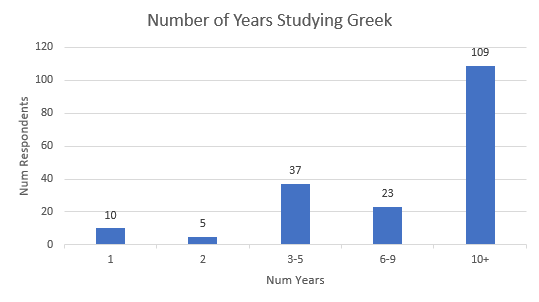
\includegraphics[width=.9\linewidth]{./images/years-studied.PNG}
\end{center}

\subsubsection{Satisfaction with current options}
\label{sec:org6bb7aa8}

\begin{center}
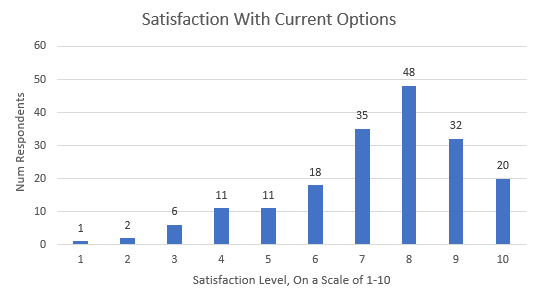
\includegraphics[width=.9\linewidth]{./images/satisfaction.PNG}
\end{center}

\subsubsection{Usage distribution of Greek entry methods}
\label{sec:orgb18d087}

\begin{center}
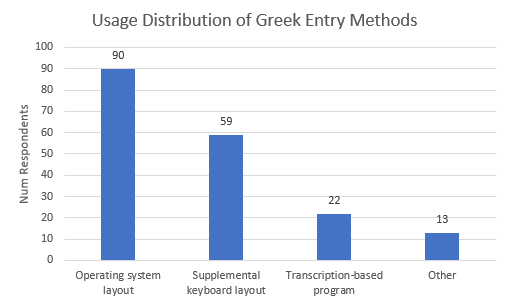
\includegraphics[width=.9\linewidth]{./images/entry-methods.PNG}
\end{center}

\subsubsection{Usage frequency of Greek entry methods}
\label{sec:org299e097}

\begin{center}
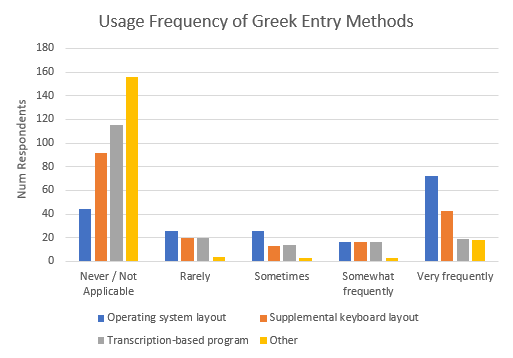
\includegraphics[width=.9\linewidth]{./images/entry-method-usage-distribution.PNG}
\end{center}

\subsubsection{Phonetic classification of primary entry method}
\label{sec:orga916eb4}

\begin{center}
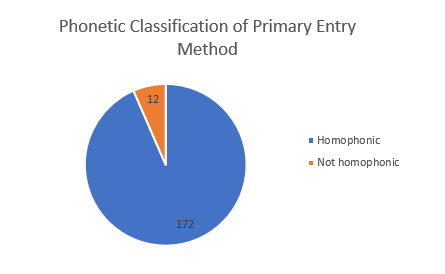
\includegraphics[width=.9\linewidth]{./images/homophonic.PNG}
\end{center}

\subsubsection{How often Greek is typed}
\label{sec:org01c195f}

\begin{center}
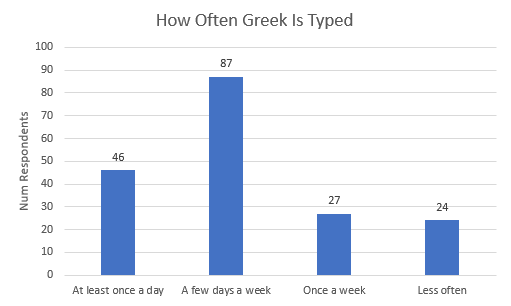
\includegraphics[width=.9\linewidth]{./images/typing-frequency.PNG}
\end{center}

\subsubsection{Typical quantity of Greek typed}
\label{sec:org69f128c}

\begin{center}
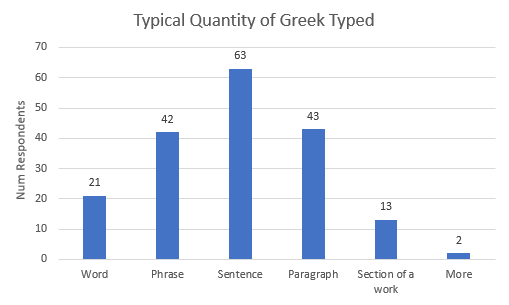
\includegraphics[width=.9\linewidth]{./images/typing-quantity.PNG}
\end{center}

\subsubsection{Preferences for entering diacritics}
\label{sec:org3fd9ebb}

\begin{center}
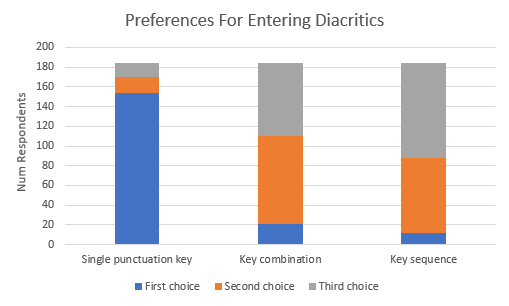
\includegraphics[width=.9\linewidth]{./images/diacritic-entry-preferences.PNG}
\end{center}

\subsubsection{Order preferences: handwriting}
\label{sec:org44375ed}

\begin{center}
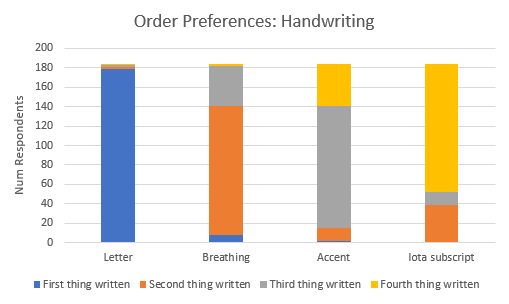
\includegraphics[width=.9\linewidth]{./images/diacritic-entry-order-writing.PNG}
\end{center}

\subsubsection{Order preferences: typing}
\label{sec:orgc2faa46}

\begin{center}
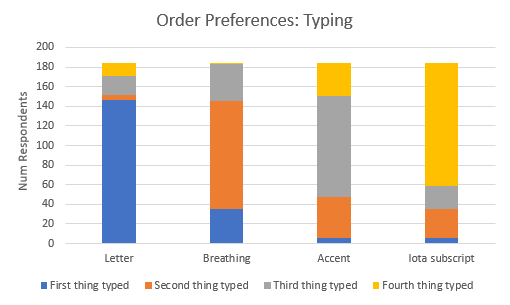
\includegraphics[width=.9\linewidth]{./images/diacritic-entry-order-typing.PNG}
\end{center}

\subsubsection{Ranking of possible features}
\label{sec:org90e5791}

\begin{center}
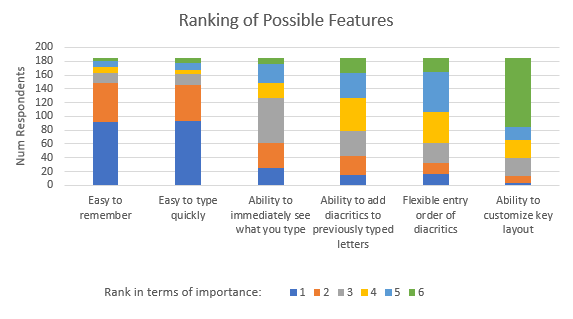
\includegraphics[width=.9\linewidth]{./images/ranking-of-possible-features.PNG}
\end{center}

\subsection{Greek layer}
\label{sec:orgaef0a0b}

\subsubsection{Graphic}
\label{sec:org645bba0}

\begin{center}
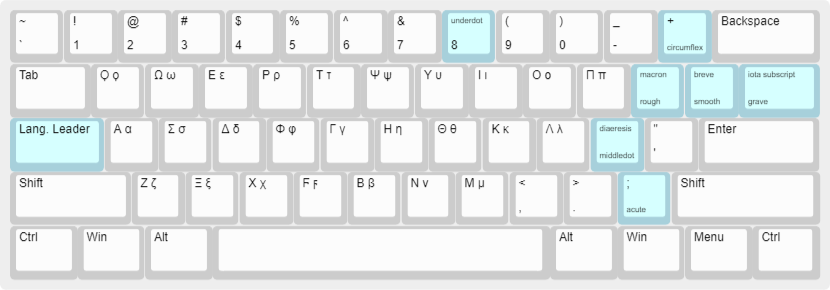
\includegraphics[width=.9\linewidth]{./images/greek-layer.png}
\end{center}

\subsubsection{Letter correspondences}
\label{sec:org0f40a12}

\begin{center}
\begin{tabular}{ll|ll}
Greek letter & English match & Greek Letter & English Match\\
\hline
Α α & A a & Ν ν & N n\\
Β β & B b & Ξ ξ & X x\\
Γ γ & G g & Ο ο & O o\\
Δ δ & D d & Π π & P p\\
Ε ε & E e & Ρ ρ & R r\\
Ζ ζ & Z z & Σ σ & S s\\
Η η & H h & Τ τ & T t\\
Θ θ & J  j & Υ υ & U u\\
Ι ι & I i & Φ φ & F f\\
Κ κ & K k & Χ χ & C c\\
Λ λ & L l & Ψ ψ & Y y\\
Μ μ & M m & Ω ω & W w\\
\end{tabular}
\end{center}

\subsubsection{Diacritics}
\label{sec:org4f6dca5}

\begin{center}
\begin{tabular}{lll}
Grouping & Diacritic & Corresponding Key\\
\hline
Breathings & Rough & [\\
 & Smooth & ]\\
Accents & Acute & /\\
 & Grave & $\backslash$\\
 & Circumflex & =\\
Quantity & Iota Subscript & \(\vert{}\)\\
 & Macron & \{\\
 & Breve & \}\\
Other & Diaeresis & :\\
 & Underdot & *\\
\end{tabular}
\end{center}

\subsubsection{Punctuation}
\label{sec:org74e4670}

\begin{center}
\begin{tabular}{ll}
Punctuation & Corresponding Key\\
\hline
Middle Dot & ;\\
Greek Question Mark & ?\\
\end{tabular}
\end{center}

\subsection{Latin-script languages}
\label{sec:org5d80c49}

Out of the box, Latin, German, French, and Spanish should work. Other Latin-script languages that only use accents (e.g., Italian) will also work.

\subsubsection{Special characters}
\label{sec:orgbdb4237}

\begin{center}
\begin{tabular}{lll}
Language & Character & Entry Sequence\\
\hline
French & ç & \{CapsLock\}c\\
 & Ç & \{CapsLock\}C\\
 & œ & \{CapsLock\}o\\
 & Π& \{CapsLock\}O\\
 & æ & \{CapsLock\}a\\
 & Æ & \{CapsLock\}A\\
German & ß & \{CapsLock\}s\\
 & ẞ & \{CapsLock\}S\\
Spanish & ñ & \{CapsLock\}n\\
 & Ñ & \{CapsLock\}N\\
 & ¿ & \{CapsLock\}?\\
 & ¡ & \{CapsLock\}!\\
\end{tabular}
\end{center}

\subsubsection{Diacritics}
\label{sec:orgffd2549}

Note that the punctuation correspondences exactly mirror those of Greek where possible. This is to keep things consistent and reduce the total memory load.

\begin{center}
\begin{tabular}{lll}
Grouping & Diacritic & Entry Sequence\\
\hline
Accents & Acute & \{CapsLock\}/\\
 & Grave & \{CapsLock\}$\backslash$\\
 & Circumflex & \{CapsLock\}=\\
Quantity & Macron & \{CapsLock\}\{\\
 & Breve & \{CapsLock\}\}\\
Other & Diaeresis/umlaut & \{CapsLock\}:\\
\end{tabular}
\end{center}

\section{Works Cited}
\label{sec:org6ef6dfb}

Chen Liao \& Pilsung Choe (2013) Chinese Keyboard Layout Design Based on Polyphone Disambiguation and a Genetic Algorithm, International Journal of Human–Computer Interaction, 29:6, 391-403, DOI: 10.1080/10447318.2013.777827 \\

Malas, Tareq M., Sinan Taifour and Gheith A. Abandah. “Toward Optimal Arabic Keyboard Layout Using Genetic Algorithm.” (2008). \\

\url{http://www.unicode.org/versions/Unicode11.0.0/ch02.pdf} \\

Mastronarde, Donald. "Before and After Unicode: Working with Polytonic Greek." Montreal APA Unicode Presentation, 2008. \\

Dhakal, V., Feit, A., Kristensson, P.O. and Oulasvirta, A. 2018. 'Observations on typing from 136 million keystrokes.' In Proceedings of the 36th ACM Conference on Human Factors in Computing Systems (CHI 2018). ACM Press. \\

Feit, Anna \& Weir, Daryl \& Oulasvirta, Antti. (2016). How We Type: Movement Strategies and Performance in Everyday Typing. 4262-4273. 10.1145/2858036.2858233. \\

E. Rumelhart, David \& Norman, Donald. (1982). Simulating a Skilled Typist: A Study of Skilled Cognitive-Motor Performance. Cognitive Science. 6. 1-36. 10.1016/S0364-0213(82)80004-9. \\

Allen, W. Sidney. 1999. Vox Graeca: a guide to the pronunciation of classical Greek. Cambridge [Cambridgeshire]: Cambridge University Press. \\

Verbrugghe, Gerald P. "Transliteration or Transcription of Greek." The Classical World 92, no. 6 (1999): 499-511. \url{doi:10.2307/4352343}. \\

Shi Min Chua and Susan J. Rickard Liow. "The Locus of Word Frequency Effects in Skilled Spelling-to-Dictation."
Quarterly Journal of Experimental Psychology. Vol 67, Issue 9, pp. 1720 - 1741. First Published September 1, 2014. \\

Bannard, Colin \& Matthews, Danielle. (2008). Stored Word Sequences in Language Learning The Effect of Familiarity on Children's Repetition of Four-Word Combinations. Psychological science. 19. 241-8. 10.1111/j.1467-9280.2008.02075.x. \\

Yamaguchi, Motonori \& D Logan, Gordon. (2016). Pushing Typists Back on the Learning Curve: Memory Chunking in the Hierarchical Control of Skilled Typewriting. Journal of experimental psychology. Learning, memory, and cognition. 42. 10.1037/xlm0000288. \\

Ghazi-Saidi L and Ansaldo AI (2017) Second Language Word Learning through Repetition and Imitation: Functional Networks as a Function of Learning Phase and Language Distance. Front. Hum. Neurosci. 11:463. doi: 10.3389/fnhum.2017.00463 \\

Dunlosky, J., Rawson, K. A., Marsh, E. J., Nathan, M. J., \& Willingham, D. T. (2013). Improving students’ learning with effective learning techniques: Promising directions from cognitive and educational psychology. Psychological Science in the Public Interest, 14, 4-58 \\

Sean HK Kang. 2016. Spaced Repetition Promotes Efficient and Effective Learning: Policy Implications for Instruction. Policy Insights from the Behavioral and Brain Sciences, Vol. 3, 1 (2016), 12--19. \\

Major, Wilfred E. "It’s Not the Size, It’s the Frequency: The Value of Using a Core Vocabulary in Beginning and Intermediate Greek." Winter 2008. \\

Nation, I. (2001). Learning Vocabulary in Another Language (Cambridge Applied Linguistics). Cambridge: Cambridge University Press. \url{doi:10.1017/CBO9781139524759}

Piantadosi, Steven T. “Zipf’s Word Frequency Law in Natural Language: A Critical Review and Future Directions.” Psychonomic bulletin \& review 21.5 (2014): 1112–1130. \\

Gu, Peter \& Keith Johnson, Robert. (1996). Vocabulary Learning Strategies and Language Learning Outcomes. Language Learning. 46. 643 - 679. 10.1111/j.1467-1770.1996.tb01355.x. \\

Raymond, Eric S. The Art of Unix Programming. Boston: Addison-Wesley, 2004.

Saltzer, J. H., and Frans Kaashoek. Principles of Computer System Design: An Introduction. Burlington, MA: Morgan Kaufmann, 2009. 
\end{document}
